\documentclass[11pt,oneside,openright]{./style/phdthesis}

\usepackage{amsmath}
\usepackage[ansinew]{inputenc}
\usepackage[portuguese]{babel}
\usepackage[printonlyused, withpage]{acronym}
\usepackage{a4wide}
\usepackage{palatino}
\usepackage{fancyhdr}
\usepackage{fancybox}
\usepackage{amssymb}
%\usepackage{chapterbib} %com este package as referencias bibliográficas aparecem no final de cada capítulo
\usepackage{cite}
\usepackage{epsfig}
%\usepackage{subfigure}
\usepackage{graphics}
\usepackage{float}
\usepackage{here}
\usepackage[T1]{fontenc}
\usepackage{rotating}
\usepackage{multirow}
%\usepackage{comment}
%\usepackage{captionhack}
\usepackage{epigraph}
\usepackage[linkcolor=black]{hyperref}
%\renewcommand{\thesubfigure}{}
\hypersetup{colorlinks=true}
\usepackage{enumerate}
%\usepackage[numbers,sort&compress]{natbib}
%\usepackage{hypernat}
\usepackage{booktabs}
\usepackage{url}                    % needed to cite a site
\usepackage{eurosym}
\usepackage{makeidx}
\usepackage{datatool}
\usepackage[toc, acronym]{glossaries}
\usepackage{graphicx}
\usepackage{caption}
\usepackage{subcaption}

\usepackage{tabulary}
\usepackage{braket}

% subfile handling packages
\usepackage{subfiles}

\usepackage{multicol} 
\usepackage{tcolorbox}
\usepackage{booktabs}




\newcommand{\onlyinsubfile}[1]{#1}
\newcommand{\notinsubfile}[1]{}
\renewcommand{\textfraction}{0.01}
\renewcommand{\topfraction}{0.99}
\renewcommand{\floatpagefraction}{0.99}
\renewcommand{\bottomfraction}{0.99}
\renewcommand{\heavyrulewidth}{1pt}
\renewcommand{\lightrulewidth}{0.50pt}
\renewcommand{\chaptername}{Capítulo}
\renewcommand{\figurename}{Figura}
\renewcommand{\appendixname}{\Large{Anexo}}
\renewcommand{\tablename}{Tabela}
\renewcommand{\acronymname}{Acrónimos}

\newcommand{\mli}[1]{\mathit{#1}}
\newcommand{\intSpace}{\!\!\!\!}
\newcommand{\doubleInt}{\!\!\int\intSpace\int\!\!}
\newcommand{\TX}{\mathit{TX}}
\newcommand{\NLI}{\mathit{NLI}}
\newcommand{\eff}{\mathit{eff}}
\newcommand{\LOASE}{\mathit{LO-ASE}}
\newcommand{\LONLI}{\mathit{LO-NLI}}
\renewcommand{\kbldelim}{[}% Left delimiter
\renewcommand{\kbrdelim}{]}% Right delimiter

%\makesavenoteenv{tabular}



\hyphenpenalty=50000
\tolerance=10000
%%% General page formatting

\oddsidemargin 0.2in
\evensidemargin 0in
%\textwidth 155mm
\headheight 15.0pt
\topmargin 0in
%\textheight 237mm

% footheight 1.0in

\makeatletter
\providecommand*{\diff}%
{\@ifnextchar^{\DIfF}{\DIfF^{}}}
\def\DIfF^#1{%
\mathop{\mathrm{\mathstrut d}}%
\nolimits^{#1}\gobblespace}
\def\gobblespace{%
\futurelet\diffarg\opspace}
\def\opspace{%
\let\DiffSpace\!%
\ifx\diffarg(%
\let\DiffSpace\relax
\else
\ifx\diffarg[%
\let\DiffSpace\relax
\else
\ifx\diffarg\{%
\let\DiffSpace\relax
\fi\fi\fi\DiffSpace}

\providecommand*{\tDeriv}[3][]{%
\frac{\diff^{#1}#2}{\diff #3^{#1}}}
\providecommand*{\pDeriv}[3][]{%
\frac{\partial^{#1}#2}%
{\partial #3^{#1}}}

\graphicspath{{./figures/}}


\DeclareMathOperator{\erf}{erf}
\DeclareMathOperator{\erfc}{erfc}
\DeclareMathOperator{\sinc}{sinc}
\DeclareMathOperator{\R}{Re}
\DeclareMathOperator{\I}{Im}
\DeclareMathOperator{\asinh}{asinh}

%\newcommand{\publ}{}

\pagenumbering{arabic} 


\makeindex

\begin{document}
%%  include the LaTeX files containing the text for each chapters

% ------------------------------------------------------------------------
\title{NetXPTO - NetPlanner}
\author{}
\date{\today}
\maketitle
% ------------------------------------------------------------------------

% ------------------------------------------------------------------------
\tableofcontents
% ------------------------------------------------------------------------


\chapter{Introduction}
\label{introduction}

The amount of traffic, in particular IP traffic, has been increasing very substantially. This increase is due to the growing number of Internet-based applications, the increase in the number of devices connected to the Internet, the expansion of optical fiber to customers' homes, increased bandwidth of mobile access technologies, and increased of video traffic \cite{cisco}.
At the same time, with the increase in traffic, operators are under heavy pressure to reduce the cost per bit transported \cite{alcatel_lucent}. This implies the introduction of new technologies, which on the one hand increase the capacity of transport of the networks and on the other, reduce the costs of operation (OPEX) \cite{opexcapex}.
This process of technological conversion is operating in a macroeconomic scenario in which operators find it difficult to finance which forces them to have strong investment constraints (CAPEX) \cite{opexcapex}.
The transport networks have been predominantly based on circuit switching, either at the level of the optical channels or at the level of the electrical circuits, and the introduction of packet switching undermines this paradigm.


\newpage
%%%%%%%%%%%%%%%%%%%%%%%%%%%%%%%%%%%%%%%%%%%%%%%%%%%%%%%%%%%%%%%%%%%%%%%%
\section{Motivation and objectives}
\label{objectives}
Taking into account all these factors, the need to implement planning tools becomes important both for suppliers and operators and is used in the various stages of the telecommunications business.
These have a very important role and directly affect the competitiveness of operators.
One of the tools used for transport network planning is the integer linear programming models.
These models offer optimal solutions, however, some scalability limitations may arise. They also allow quick and easy changes.
Therefore this model becomes relevant in an environment where requirements may differ substantially between operators \cite{teserui}.\\
Due to the importance of transport network planning and design, this dissertation aims to achieve the following main objectives:

\begin{enumerate}
  \item Define one reference network and three different scenarios for performing tests.
  \item Develop ILP models for opaque, transparent and translucent networks without survivability and using 1+1 protection.
  \item Get analytical solutions for the previous point.
  \item Compare the analytical results and results based on ILP with the results obtained through heuristics.
\end{enumerate}


%%%%%%%%%%%%%%%%%%%%%%%%%%%%%%%%%%%%%%%%%%%%%%%%%%%%%%%%%%%%%%%%%%%%%%%%%%%%%%%%%%%%%%%
\section{Thesis outline}
\label{outline}

This thesis is organized in 7 chapters. Chapter \ref{chap_reference_network} consists of a state-of-art review about optical transport networks. In this chapter is also where the reference network used throughout the dissertation as well as the different traffics used is defined. The Chapter \ref{chap_capex} begins by determining the CAPEX calculation formula for use in the ILP model and for analytical calculations. The first section refers to ILP models and the other to analytical models. In Chapter \ref{chap_ilp} are several sections each for a particular mode of transport and certain survivability. In section \ref{ILP_Opaque_Survivability} we have opaque without survivability, in section \ref{ILP_Opaque_Protection} opaque with 1+1 protection. Sections \ref{ILP_Transp_Survivability} and \ref{ILP_Transp_Protection} relate to the transparent and lastly sections \ref{ILP_Transluc_Survivability} and \ref{ILP_Transluc_Protection} refer to the translucent. In the referred section it is possible to see the model description, the detailed description of the results and the conclusions of these results. The analytical calculation of all the models referred to in Chapter \ref{chap_ilp} can be found in Chapter \ref{chap_analytical}. In Chapter \ref{chap_comparative} the results obtained throughout this dissertation are compared and the chapter is divided into six sections where each corresponds to a certain mode of transport with their respective survivability. The last step is the conclusions \ref{chap_conclusions} and suggestions for future research directions.

%%%%%%%%%%%%%%%%%%%%%%%%%%%%%%%%%%%%%%%%%%%%%%%%%%%%%%%%%%%%%%%%%%%%%%%%%%%%%%%%%%%%%%%%%%%%%%%%%%%%%%%%%%%%%%%%%%%%%%%%%%%%%

% References
\phantomsection
\addcontentsline{toc}{section}{References}
%
\renewcommand{\bibname}{References}
%\bibliographystyle{IEEEtran}
%\bibliography{rmorais}
%
%
% Generated by IEEEtran.bst, version: 1.13 (2008/09/30)
\begin{thebibliography}{10}
\providecommand{\url}[1]{#1}
\csname url@samestyle\endcsname
\providecommand{\newblock}{\relax}
\providecommand{\bibinfo}[2]{#2}
\providecommand{\BIBentrySTDinterwordspacing}{\spaceskip=0pt\relax}
\providecommand{\BIBentryALTinterwordstretchfactor}{4}
\providecommand{\BIBentryALTinterwordspacing}{\spaceskip=\fontdimen2\font plus
\BIBentryALTinterwordstretchfactor\fontdimen3\font minus
  \fontdimen4\font\relax}
\providecommand{\BIBforeignlanguage}[2]{{%
\expandafter\ifx\csname l@#1\endcsname\relax
\typeout{** WARNING: IEEEtran.bst: No hyphenation pattern has been}%
\typeout{** loaded for the language `#1'. Using the pattern for}%
\typeout{** the default language instead.}%
\else
\language=\csname l@#1\endcsname
\fi
#2}}
\providecommand{\BIBdecl}{\relax}
\BIBdecl

\bibitem{cisco}
Cisco, ``Global Mobile Data Traffic Forecast Update 2015-2020,'' in \emph{Cisco Visual Networking Index}, pp. 2,3, 2016.

\bibitem{alcatel_lucent}
\BIBentryALTinterwordspacing
Alcatel-Lucent (2009). ``The new economics of telecom networks - bringing value back to the network,'' Tech. Rep. [Online]. Available:
  \url{http://images.tmcnet.com/online-communities/ngc/pdfs/application-enablement/whitepapers/The-New-Economics-of-Telecom-Networks.pdf}
\BIBentrySTDinterwordspacing

\bibitem{opexcapex}
S.~Verbrugge, D.~Colle, M.~Pickavet, P.~Demeester, S.~Pasqualini, A.~Iselt, A.~Kirst\"{a}dter, R.~H\"{u}lsermann, F.-J. Westphal, and M.~J\"{a}ger, ``Methodology and input availability parameters for calculating OpEx and CapEx costs for realistic network scenarios,'' \emph{Journal of Optical Networking}, vol.~5, no.~6, pp. 509--520, June 2006.

\bibitem{teserui}
R.~M.~D. Morais, ``Planning and Dimensioning of Multilayer Optical Transport Networks.'' PhD thesis, Universidade de Aveiro, 2015.

\end{thebibliography}


% ------------------------------------------------------------------------
\chapter{Simulator Structure}

LinkPlanner is a signals open-source simulator.

The major entity is the system.

A system comprises a set of blocks.

The blocks interact with each other through signals.

\section{System}

\section{Blocks}

\section{Signals}

List of available signals:

\begin{itemize}
    \item Signal

\end{itemize}










% ------------------------------------------------------------------------
\chapter{Development Cycle}

The NetXPTO-LinkPlanner has been developed by several people using git as a version control system.
The NetXPTO-LinkPlanner repository is located in the GitHub site http://github.com/netxpto/linkplanner.
The more updated functional version of the software is in the branch master.
Master should be considered a functional beta version of the software.
Periodically new releases are delivered from the master branch under the branch name Release<Year><Month><Day>.
The integration of the work of all people is performed by Armando Nolasco Pinto in the branch Develop.
Each developer has is how branch with his/her name.





% ------------------------------------------------------------------------
\chapter{Case Studies}

\clearpage

\begin{tcolorbox}	
\begin{tabular}{p{2.75cm} p{0.2cm} p{10.5cm}} 	
\textbf{Student Name}  &:& Tiago Esteves\\
\textbf{Starting Date} &:& October 03, 2017\\
\textbf{Goal}          &:& Implement the dimensioning of optical networks in the translucent transport mode.
\end{tabular}
\end{tcolorbox}

\section{Objective and methodology for the dissertation}

\subsection{Objective}
The objective of this dissertation is to develop ILP and Heuristic models for networks with translucent transport mode and finally integral in net2plan.
To achieve this goal, the following steps must be:
\begin{itemize}
  \item Develop ILP models for opaque, transparent and translucent networks using 1 + 1 protection.
  \item Obtain a solution for network through heuristic algorithms.
  \item Compare and validate the results obtained through the heuristics with the results based on ILP.
\end{itemize}

\subsection{Methodology}
The methodology used in this dissertation is to define two networks (a reference network and another realistic network) and then apply the ILPs to the reference network and to the realistic network.
Subsequently we will develop heuristics that will be generated in Net2Plan and validated based on the comparison with the results obtained from the ILPs.
In addition to being used two networks will also be applied two possible scenarios being one of them with little traffic and the other with much traffic.

This procedure will be done as follows:
\begin{enumerate}
  \item Opaque with 1+1 Protection
  \item Transparent with 1+1 Protection
  \item Translucent with 1+1 Protection
\end{enumerate}

\section{Physical Network Topology}

\subsection{Reference Network}
As we can see in the figure, our reference network consists of 6 nodes and 8 Bidirectional links.
The average length of the links was chosen so that the following calculations are more simplistic.

\begin{figure}[h!]
\centering
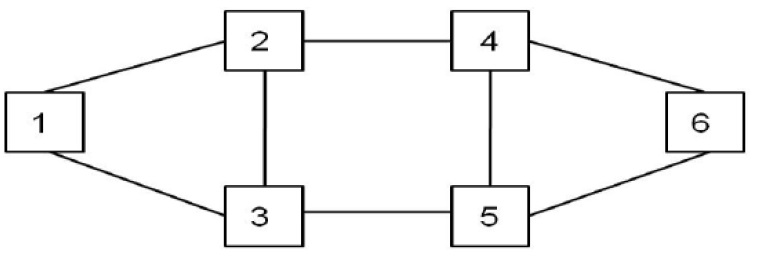
\includegraphics[width=\textwidth]{RedeTeste}
\caption{Physical Topology of the Reference Network.}
\end{figure}

\vspace{10pt}

The following table shows the values of the variables associated with this network.
\begin{table}[h!]
\vspace{10pt}
\centering
\begin{tabular}{|| c | c | c||}
 \hline
 Constant & Description & Value \\
 \hline\hline
 N & Number of Nodes & 6 \\
 L & Number of Bidirectional Links & 8 \\
 <$\delta$> & Node out-degree & 2,667 \\
 <len> & Mean Link Length (km) & 500 \\
 <h> & Mean Number of Hops,for Working Paths & 1,533 \\
 <h'> & Mean Number of Hops,for Backup Paths & 2,467 \\
 \hline
\end{tabular}
\caption{Table of reference network values}
\label{table:1}
\end{table}
\vspace{10pt}

As we can see from table \ref{table:1}, to do all the calculations necessary for this project, let us know the value of the traffic used. This value is defined depending on the scenario used, as we can see:
\begin{itemize}
  \item Shortly Traffic: \textbf{0.5 TBits/s}
  \item Very Traffic: \textbf{5 TBits/s}
\end{itemize}
\vspace{10pt}

\subsection{Realistic Network}
The real network chosen for this work is the EON (European Optical Network).
The way the nodes are arranged geographically can be seen from the following figure.
\vspace{100pt}

\begin{figure}[h!]
\centering
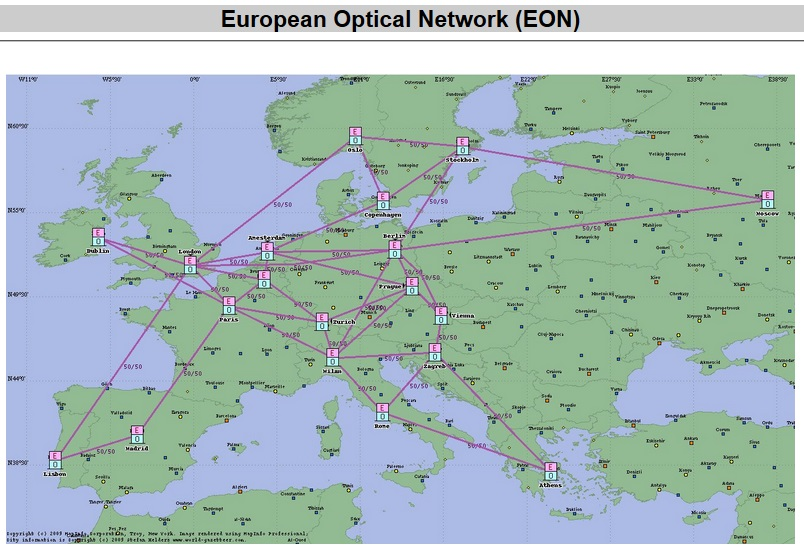
\includegraphics[width=\textwidth]{EON_Rede_Realista}
\caption{Physical Topology of the Realistic Network.}
\end{figure}

The table \ref{table:2} shows the values of the variables associated with this network.
\begin{table}[h!]
\centering
\begin{tabular}{|| c | c | c||}
 \hline
 Constant & Description & Value \\
 \hline\hline
 N & Number of Nodes & 19 \\
 L & Number of Bidirectional Links & 37 \\
 <$\delta$> & Node out-degree & 3,89 \\
 <len> & Mean Link Length (km) & 753,76 \\
 <h> & Mean Number of Hops,for Working Paths & 2,3 \\
 <h'> & Mean Number of Hops,for Backup Paths & 3,2 \\
 \hline
\end{tabular}
\caption{Table of realistic network values}
\label{table:2}
\end{table}
\vspace{10pt}

Again, to make all the necessary calculations, only the value of the traffic used is missing. This value is set depending on the scenario used, as we can see:

\begin{itemize}
  \item Shortly Traffic: \textbf{2 TBits/s}
  \item Very Traffic: \textbf{20 TBits/s}
\end{itemize}
\vspace{10pt}

\section{Dimensioning using ILP models}

\subsection{Opaque with 1+1 Protection}
The objective function of following ILP is a minimization of the sum of two variables: total number of flows crossing link (i; j) for all demand pairs (o; d) and total number of optical channels in each link (i; j).
\begin{figure}[h!]
  \centering
  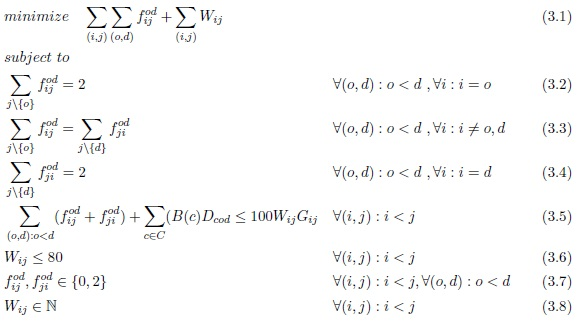
\includegraphics[scale=1]{ILP_Opaque}
\end{figure}

The objective function, to be minimized, is the expression(3.1). The flow conservation constraints are (3.2), (3.3) and (3.4). First constraint ensures that, for all demand pairs (o,d), it routes two flows of traffic for all bidirectional links (i,j) when "j" is not equal to the origin of the demand. Equation (3.4) is based on the same idea of (3.1), however applied in reverse direction. Assuming bidirectional traffic, so the number of flows in both directions of the link is the same (3.3). The inequality (3.5) is considered grooming constraint, so it means the total client traffic flows can not be greater than the capacity of optical channels on all links. Another important constraint (3.6) is the capacity of the optical channels which must be less or equal to 100 Gb/s or 80 ODU0. The number of flows per demand can be zero if there are no traffic demands or two if considering working and protection traffic (3.7). The last constraint is just needed to ensure the number optical of channels is a positive integer values greater than zero.

\subsection{Transparent with 1+1 Protection}

The optimization model suggested for transparent transport mode with dedicated path protection intends to minimize the total number of flows crossing link (i; j) for all demand pairs (o; d). The mathematical model described below also minimizes the total number of optical channels between each demand end nodes Wod, instead of minimizing the number of optical link-by-link channels as in the previous model.

\begin{figure}[h!]
  \centering
  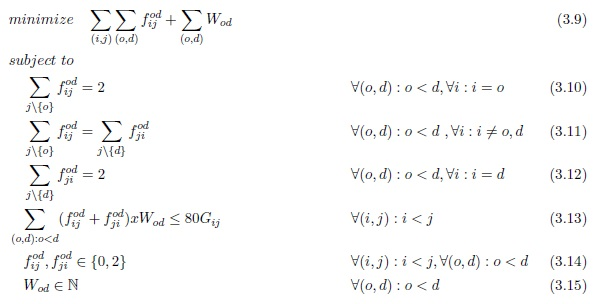
\includegraphics[scale=1]{ILP_Transp}
\end{figure}

The objective function, to be minimized, is the expression(3.9). The flow conservation is performed by equations (3.10), (3.11) and (3.12) and share the same mathematical description of opaque model. The inequality (3.13) answers capacity constraint problem. Then, total flows times the traffic of the demands must be less or equal to the capacity of network links. The grooming of this model can be done before routing since the traffic is aggregated just for demands between the same nodes, thus not depending on the routes. Last two constraints define the total number of flows must be zero if there is no demand, or two for a demand with traffic protection, and the number of optical channels must be a counting number.

\subsection{Translucent with 1+1 Protection}

\section{ILP Results}
In this initial phase the results will be presented using ILP to calculate the CAPEX of the reference network.
For this we will use the following calculation formulas:

\begin{figure}[h!]
  \centering
  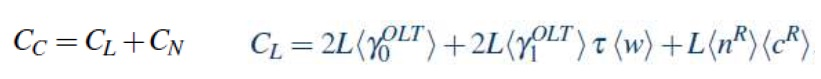
\includegraphics[width=\textwidth]{CAPEX}
  \caption{First function is CAPEX cost, second is cost of the links}
\end{figure}

\begin{figure}[h!]
  \centering
  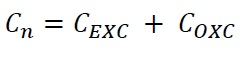
\includegraphics[scale=1]{CAPEX2}
  \caption{This function represent the cost of the nodes}
\end{figure}

We will also need a price list that we can see below.

\begin{figure}[h!]
  \centering
  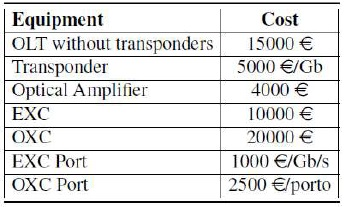
\includegraphics[scale=1]{TabValor}
  \caption{Table with costs}
\end{figure}

Finally we will calculate the CAPEX values for the various situations mentioned.

\subsection{Opaque with 1+1 Protection}
First we will present the scenario of little traffic and then in the case of a lot of traffic.
To know the value of CAPEX we will have to first calculate the value of the cost of the links and then the cost of the nodes.

\textbf{First scenario:}

Through the table, of auxiliary calculations and MatLab the value of the cost of the links is:

Cost link = 24 336 000 euros

Again, through the table, of auxiliary calculations and MatLab the value of the cost of the nodes is:

Cost node = 5 860 000 euros

Finally, for this scenario the cost of CAPEX is:

CAPEX = 30 196 000 euros

\textbf{Second scenario:}

Cost link = 191 336 000 euros

Cost node = 48 260 000 euros

CAPEX = 239 596 000 euros

\subsection{Transparent with 1+1 Protection}
Again, the first we will present the little traffic and then the lot of traffic.
To know the value of CAPEX we will have to first calculate the value of the cost of the links and then the cost of the nodes.

\textbf{First scenario:}

Through the table, of auxiliary calculations and MatLab the value of the cost of the links is:

Cost link = 44 336 000 euros

Again, through the table, of auxiliary calculations and MatLab the value of the cost of the nodes is:

Cost node = 2 515 000 euros

Finally, for this scenario the cost of CAPEX is:

CAPEX = 46 851 000 euros

\textbf{Second scenario:}

Cost link = 391 336 000 euros

Cost node = 21 445 000 euros

CAPEX = 412 781 000 euros

\subsection{Translucent with 1+1 Protection}

\section{Heuristics}







%\section{Continuous Variable Quantum Transmission System}
%
%\subfile{./sdf/cv_system/cv_system}


%\include{sdf/cv_system/cv_system}
%\include{../sdf/TexFiles/EnquadramentoVHDL}
%\include{CapacidadeTeoriacadeTransmitirInformacao}
%\include{SistemasCoerentesComDSP}
%\include{SistemasMultiMode}
%\include{SistemasComunicacaoQuanticos}
%\include{Conclusao}
%\appendix
%\include{Acronymous}
%\printindex

%   create the appendix and include it


\pagebreak

%--------------------------------- SECTION ----------------------------------
\bibliographystyle{ieeetr}
% argument is your BibTeX string definitions and bibliography database(s)
%\bibliography{../../../Computadores/Bibtex/IEEEabrv,../../../Computadores/Bibtex/AnpBib}


\printglossaries

\end{document}
